\newcommand{\booktitle}{用户手册}
\newcommand{\tocname}{目录}
\newcommand{\figword}{图}
\newcommand{\chapterword}{第 \thesection\ 章}
\newcommand{\coverline}{一维输出数据的读取、绘图与导出}
\newcommand{\covercaption}{横轴为网格中心位置，单位为微米。三条曲线取自本手册的合成示例，展示同一个温度峰在三个输出时刻的位置。}
\newcommand{\editionline}{桌面版 \enspace 2.3.1}
\newcommand{\manualdate}{2026 年 11 月}
\newcommand{\creditline}{简体中文版 \enspace ·\enspace 软件作者 徐博}
% Compile either edition from its own directory with XeLaTeX.
\documentclass[11pt,a4paper]{article}
\usepackage[top=22mm,bottom=23mm,left=22mm,right=22mm,headheight=16pt,footskip=12mm]{geometry}
\usepackage{fontspec,xeCJK}
\setmainfont{TeX Gyre Pagella}
\setsansfont{TeX Gyre Heros}
\setmonofont[Scale=0.88]{Latin Modern Mono}
\IfFileExists{C:/Windows/Fonts/msyh.ttc}
  {\setCJKmainfont[AutoFakeBold=2]{SimSun}\setCJKsansfont{Microsoft YaHei}\setCJKmonofont{Microsoft YaHei}}
  {\setCJKmainfont[BoldFont=FandolSong-Bold.otf]{FandolSong-Regular.otf}%
   \setCJKsansfont[BoldFont=FandolHei-Bold.otf]{FandolHei-Regular.otf}\setCJKmonofont{FandolHei-Regular.otf}}
\usepackage{graphicx,xcolor,booktabs,tabularx,array,enumitem,fancyhdr,tikz}
\usepackage{hyperref}
\definecolor{ink}{HTML}{182F40}
\definecolor{teal}{HTML}{006D72}
\definecolor{muted}{HTML}{425B66}
\definecolor{rulecol}{HTML}{B6D0CF}
\definecolor{wash}{HTML}{EEF5F4}
\hypersetup{unicode=true,colorlinks=true,linkcolor=teal,urlcolor=teal,bookmarksnumbered=true,bookmarksdepth=2,
 pdfauthor={MULTI1Dvisual},pdftitle={MULTI1Dvisual 2.3.1 — \booktitle}}
\urlstyle{same}
\setlength{\parindent}{0pt}
\setlength{\parskip}{5.5pt}
\linespread{1.10}
\setlist[enumerate]{leftmargin=1.9em,label=\textcolor{teal}{\sffamily\bfseries\arabic*.},itemsep=3pt,topsep=4pt,parsep=0pt}
\setcounter{tocdepth}{1}
\renewcommand{\contentsname}{\tocname}
\pagestyle{fancy}\fancyhf{}
\fancyhead[L]{\small\sffamily\bfseries\color{teal}MULTI1Dvisual}
\fancyhead[R]{\small\sffamily\color{muted}\nouppercase{\leftmark}}
\fancyfoot[L]{\footnotesize\sffamily\color{muted}\booktitle\enspace ·\enspace 2.3.1}
\fancyfoot[R]{\sffamily\bfseries\color{teal}\thepage}
\renewcommand{\headrulewidth}{0.4pt}
\renewcommand{\headrule}{{\color{rulecol}\hrule height \headrulewidth width\headwidth}}
\raggedbottom
\setlength{\emergencystretch}{2em}
\newcommand{\chapterpage}[2]{\clearpage\refstepcounter{section}\label{#1}%
 \addcontentsline{toc}{section}{\protect\numberline{\thesection}#2}\markboth{#2}{}%
 {\sffamily\bfseries\color{teal}\chapterword\par}\vspace{0.5mm}
 {\sffamily\bfseries\color{ink}\fontsize{24}{30}\selectfont #2\par}\vspace{2mm}}
\newcommand{\nextpage}[2]{\clearpage\phantomsection\label{#1}%
 \pdfbookmark[2]{#2}{sub:#1}%
 {\sffamily\bfseries\color{teal}\chapterword\par}\vspace{0.5mm}
 {\sffamily\bfseries\color{ink}\fontsize{22}{28}\selectfont #2\par}\vspace{2mm}}
\newcommand{\subhead}[1]{\par\addvspace{2.5mm}{\large\sffamily\bfseries\color{teal}#1\par}\nobreak}
\newcommand{\ui}[1]{{\sffamily\bfseries\color{ink}#1}}
\newcommand{\code}[1]{{\ttfamily\detokenize{#1}}}
\newcommand{\keys}[1]{{\small\sffamily\bfseries #1}}
\newcommand{\checknote}[2]{\par\addvspace{2.5mm}\noindent\colorbox{wash}{%
 \parbox{\dimexpr\linewidth-2\fboxsep\relax}{\vspace{1mm}\hspace{1.4mm}%
 \begin{minipage}{\dimexpr\linewidth-3mm\relax}{\sffamily\bfseries\color{teal}#1}\enspace #2\end{minipage}\vspace{1.4mm}}}\par}
\newcommand{\Table}[3]{\par\smallskip\begingroup\small\renewcommand{\arraystretch}{1.24}%
 \begin{tabularx}{\linewidth}{@{}>{\raggedright\arraybackslash}p{.295\linewidth}>{\raggedright\arraybackslash}X@{}}\toprule
 \sffamily\bfseries\color{teal}#1 & \sffamily\bfseries\color{teal}#2\\\midrule #3\bottomrule
 \end{tabularx}\endgroup\par}
\newcounter{manualfig}
\newcommand{\Figure}[3]{\par\addvspace{2mm}\stepcounter{manualfig}\begingroup\centering
 \includegraphics[width=\linewidth,height=#3,keepaspectratio]{images/#1.png}\par
 \endgroup{\small\color{muted}{\sffamily\bfseries\color{teal}\figword\ \themanualfig.}\enspace #2\par}\smallskip}
\newcommand{\repo}{\href{https://github.com/boxu-pku/MULTI1Dvisual}{GitHub · boxu-pku/MULTI1Dvisual}}
\newcommand{\cover}{\thispagestyle{empty}\vspace*{6mm}
 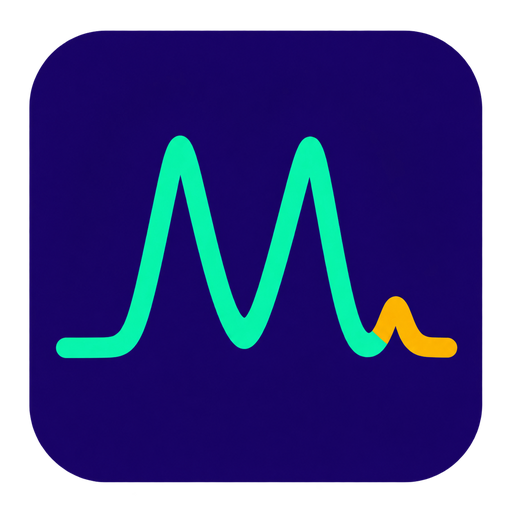
\includegraphics[width=27mm]{../../resources/icons/multi1dvisual.png}\par\vspace{9mm}
 {\sffamily\bfseries\color{ink}\fontsize{38}{44}\selectfont MULTI1Dvisual\par}
 {\sffamily\bfseries\color{teal}\fontsize{28}{37}\selectfont\booktitle\par}
 \vspace{3mm}{\Large\color{muted}\coverline\par}
 \vfill
 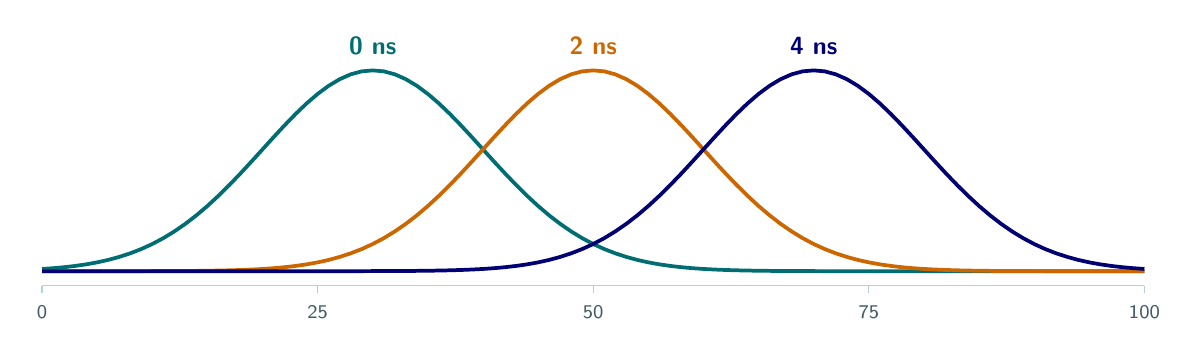
\begin{tikzpicture}[x=.140cm,y=.51cm]
 \draw[rulecol] (0,0)--(100,0);
 \foreach \p in {0,25,50,75,100} {
  \draw[rulecol] (\p,0)--(\p,-.18);
  \node[below,font=\scriptsize\sffamily,text=muted] at (\p,-.25){\p};}
 \foreach \p/\col/\name in {30/teal/0,50/orange!80!black/2,70/blue!45!black/4}{
  \draw[line width=1.35pt,color=\col] plot[domain=0:100,samples=101] (\x,{.36+5*exp(-((\x-\p)^2)/200)});
  \node[above,font=\small\sffamily\bfseries,text=\col] at (\p,5.52){\name\ ns};}
 \end{tikzpicture}\par
 {\small\color{muted}\covercaption\par}
 \vfill{\color{rulecol}\rule{\linewidth}{0.8pt}}\par
 {\large\sffamily\bfseries\color{ink}\editionline}\hfill{\sffamily\color{muted}\manualdate}\par
 {\small\color{muted}\creditline}\clearpage}
\newcommand{\contentspage}{\markboth{\tocname}{}\pdfbookmark[1]{\tocname}{contents}%
 \tableofcontents}

\begin{document}\color{ink}
\cover
\contentspage
\subhead{如何使用这本手册}
初次使用可按第~\ref{quick}~章打开练习数据。要按任务查找工具，可直接翻到第~\pageref{tools}~页。冲击波检测的完整练习从第~\pageref{shock}~页开始。
\checknote{练习材料}{项目首页与桌面安装包均提供两版共用的 \code{quickstart.zip}。冲击波检测的截图来自 Ubuntu 中文界面，其余桌面截图来自 Windows。部分工具的坐标、图例和选项保留英文名称。}
\chapterpage{install}{安装桌面版}
\subhead{Linux 图形安装}
按发行版选择安装包。安装完成后，系统会登记桌面图标和应用菜单入口。Python、Qt 和绘图库由发行版的软件包管理器提供，请允许它获取并安装列出的依赖。
\Table{使用的系统}{2.3.1 版安装文件}{
Debian 或 Ubuntu & \code{multi1dvisual_2.3.1-1_all.deb}\\
Fedora & \code{multi1dvisual-2.3.1-1.noarch.rpm}\\}
\begin{enumerate}
\item 在文件管理器中双击下载好的安装包。如果看到的是文件列表，右键选择“打开方式”，改用系统的软件安装器。在装有 GDebi 的 Ubuntu 上也可以选 GDebi。
\item 在安装窗口核对包名 \code{multi1dvisual}，点击“安装”。系统级安装可能会提示输入管理员密码。
\item 在应用菜单搜索 \ui{MULTI1Dvisual}，点击图标启动。也可以在图形桌面的终端输入 \code{multi1dvisual}。
\item 看到三个绘图标签页后，从\ui{帮助 → 使用文档}选择中文版或英文版，即可用本机 PDF 阅读器离线打开。
\end{enumerate}
\subhead{用终端安装}
在存放下载文件的目录中打开终端。Debian 或 Ubuntu 执行第一条命令，Fedora 执行第二条。文件名前的 \code{./} 表示安装当前目录中的文件。
\begin{verbatim}
sudo apt install ./multi1dvisual_2.3.1-1_all.deb
\end{verbatim}
\begin{verbatim}
sudo dnf install ./multi1dvisual-2.3.1-1.noarch.rpm
\end{verbatim}
\subhead{核对版本、升级和卸载}
用 \code{dpkg-query -W multi1dvisual} 可查看 Debian 或 Ubuntu 上的安装版本。在 Fedora 上使用 \code{rpm -q multi1dvisual}。升级时将安装命令中的文件名换成新版本。需要卸载时，分别使用 \code{sudo apt remove multi1dvisual} 或 \code{sudo dnf remove multi1dvisual}。
\checknote{找到练习文件}{Linux 安装版把手册和示例放在 \code{/usr/share/multi1dvisual/docs/} 下。先把其中的 \code{examples/quickstart.zip} 复制到自己可写的目录，再解压练习。}

\nextpage{otherinstall}{Windows 安装与从源码启动}
\subhead{Windows 10 或 11，x64}
\begin{enumerate}
\item 打开 \code{MULTI1Dvisual-Setup-2.3.1-x64.exe}。选择安装界面语言，根据需要勾选桌面快捷方式。
\item 完成向导后，在“开始”菜单启动 \ui{MULTI1Dvisual}。安装包内含 Python 运行环境及绘图依赖。
\item 从\ui{帮助 → 使用文档}打开 PDF。若使用默认安装位置，在资源管理器地址栏输入 \texttt{\%LOCALAPPDATA\%}，再进入 \code{Programs/MULTI1Dvisual/manual/docs}。其中的 \code{examples} 目录有练习压缩包。
\end{enumerate}
自定义安装目录下的文档位于 \code{manual/docs}。需要卸载时，在 Windows 设置的“已安装的应用”中找到 MULTI1Dvisual。
\subhead{在 Linux 上从源码启动}
在有桌面显示的终端中，进入同时包含 \code{main.py} 和 \code{requirements.txt} 的项目根目录。确保所用 Python 支持 \code{venv}，然后用下面的命令启动程序。
\begin{verbatim}
python3 -m venv .venv
. .venv/bin/activate
python -m pip install -r requirements.txt
python main.py
\end{verbatim}
源码中的两份 PDF 分别位于 \code{docs/manual_CN} 和 \code{docs/manual_EN}。练习包在 \code{docs/examples} 下。从源码制作桌面安装包的步骤见仓库内的 \code{packaging/README.md}。
\subhead{切换主界面语言}
打开\ui{帮助 → 更改语言}，选择“简体中文”或 \ui{English}，确认后重启程序。英文界面下同一命令位于 \ui{Help → Change Language}。安装向导和应用主窗口分别保存各自的语言选择。
\checknote{第一次打开}{主窗口初始显示空画布。按 \keys{Ctrl+O} 载入数据后，还需要选择变量并点击“绘制”。下一页可以从头完成一次完整操作。}

\chapterpage{quick}{用示例完成第一张图}
把 \code{quickstart.zip} 解压到可写目录。示例提供同一组数据的十进制和二进制文件。网格保持静止，温度峰随时间平移，方便在不同绘图页交叉核对同一个数值。
\begin{enumerate}
\item 按 \keys{Ctrl+O}，打开 \code{quickstart.case}，两个同名开头的 \code{.dat} 文件保存在旁边。文件信息栏应显示 \ui{9} 个时间步、\ui{21} 个网格。
\item 按 \keys{Ctrl+1} 进入“空间图”。选择变量 \ui{T}、坐标 \ui{XC}、位置单位 \ui{um} 和数值单位 \ui{eV}。按住 Ctrl 依次选中第 \ui{\#0}、\ui{\#4}、\ui{\#8} 个时刻，点击\ui{绘制}。三条曲线的峰位依次向右移动。
\item 按 \keys{Ctrl+2}，选择网格单元的时间演化模式，再选 \ui{T} 和 \ui{Cell \#10}。时间设为 \ui{ns}、温度设为 \ui{eV}，点击\ui{绘制}。该单元在 2 ns 达到最高温度。
\item 按 \keys{Ctrl+3}，在热图中选 \ui{T}、\ui{XC}，横轴设为时间。在颜色设置中选 \ui{viridis}，点击颜色范围旁的“自动”，然后绘制。最亮的区域从约 30 µm 移到 70 µm。
\item 回到空间图，保留三个时刻，点击本页的\ui{导出数据}，保存为 \code{profiles.csv}。逐列核对下表。若需要图像，再按 \keys{Ctrl+S}，输入带 \code{.png} 后缀的文件名。
\end{enumerate}
\Table{时刻编号和时间}{离散网格上的 T 最大值}{
\#0 \enspace 0.0 ns & 30 µm 处为 8 eV，对应第 \#6 个单元\\
\#4 \enspace 2.0 ns & 50 µm 处为 8 eV，对应第 \#10 个单元\\
\#8 \enspace 4.0 ns & 70 µm 处为 8 eV，对应第 \#14 个单元\\}
\subhead{认识练习数据}
9 个输出时刻相隔 0.5 ns。21 个单元中心从 0 到 100 µm，间隔 5 µm。\code{T} 是叠加在 2 eV 基线上的平滑温度峰，\code{R} 是随位置缓慢增加的密度。全局标量 \code{ENIE} 从 10 增加到 18，此处使用示例的存储数值。
\checknote{其他练习文件}{\code{quickstart.out} 以二进制保存相同的温度数据，供第~\ref{recorder}~章录制回放。单独的 \code{moving-edge/} 文件夹提供密度示例，用于第~\ref{shock}~章的冲击波检测和第~\ref{standard}~章的标准出图。}

\chapterpage{files}{打开文件与使用主窗口}
\Table{打开的入口}{文件之间的关系与读取方式}{
\code{fort.10} 或二进制 \code{.out} & 直接打开输出文件即可读取各时间步存储的坐标、场量和时间。\\
格式化文本 \code{fort.10} & 程序检查起始记录，区分支持的 MULTI-IFE 格式化文本和标准二进制输出。建议保留原始文件名。\\
\code{name.case} & 同一目录下必须同时有 \code{name.scalars.dat} 和 \code{name.center.dat}。名称前缀必须一致。\\
可选的 ASCII 表 & \code{name.interface.dat} 提供界面位置及界面量。有群数据时，还可能包含 \code{name.group.dat}。\\}
\subhead{检查十进制文件}
练习数据的列之间使用制表符。以 \texttt{\# TIME} 开始的表头给出列名。标量表每个输出时刻一行。中心量按时间分块，同一块内按网格顺序排列，每个时间块的行数相同。程序按行数将其重排成数组。在电子表格中单独排序某一列，可能使物理量与网格错位。
\subhead{从主窗口辨认当前数据}
顶部信息栏显示当前文件名、时间步数和网格数。每个标签页的左侧为选项，右侧为图形。窗口高度较小时，可滚动左侧面板找到“绘制”和“导出数据”。窗口底部的状态行显示最近一次载入、绘图或保存的结果。
\begin{enumerate}
\item 用 \keys{Ctrl+O} 打开选取窗口。即使按钮写着“打开二进制文件”，文件过滤器也支持 \code{.case}。
\item 如果磁盘上的输出已更新，点击信息栏或工具栏中的 \ui{Reload}。重新选择变量和时间步，再次绘制。
\item 打开第二个文件后，当前数据会切换。导出或开始录制前先核对顶部文件名。
\end{enumerate}
\checknote{重新打开数据}{旧式 ASCII 导出会生成 \code{_SCout.txt} 和 \code{_TSout.txt}。要读取十进制算例，应选择原始的 \code{.case} 及其配套 \code{.dat} 文件。}

\nextpage{coords}{选择坐标与单位}
先确定要固定什么量。空间图固定输出时刻，网格时间曲线固定数组中的单元编号。在运动网格上，固定空间位置的截面可能随时间穿过不同单元。
\Table{坐标系}{含义与用法}{
\code{XC} / \code{X} & 当前时刻的单元中心／界面位置，单位为长度。网格随时间运动时，各时间步的位置可以不同。\\
\code{LC} / \code{LI} & 初始输出时刻的中心／界面位置。后续记录仍沿用初始长度坐标，便于跟踪同一编号。\\
\code{NC} / \code{NI} & 文件中记录的单元／界面编号，单位为 index。该编号可能与从零开始显示的 \ui{Cell \#} 列表相差一。\\
\code{CMC} / \code{CMI} & 中心／界面上的累积质量坐标，在文件提供相应数据时可用，量纲为单位面积质量。\\}
菜单根据文件中已有或可推得的坐标生成。中心量通常有 \(N\) 个值，界面量通常有 \(N+1\) 个值。比较中心温度时选 \code{XC}。若某变量存储在界面上，选 \code{X} 并检查数组长度，再判断最外侧的数据。
\subhead{分别辨认横轴、纵轴和颜色条}
界面上的 \code{um} 表示微米。1 cm 等于 \(10^4\) µm，1 ns 等于 \(10^{-9}\) s。\code{T}、\code{TI}、\code{TR} 可以在 eV 和 K 间切换，程序使用 1 eV 对应 11,604.518 K。练习峰值 8 eV 约合 92,836 K。\code{P}、\code{PT} 的压强单位可选 GPa、Mbar 和原始单位 \code{dyn/cm^2}。改变某一项时，应分别读出坐标单位和数值单位。
\subhead{同一位置为何会有两个编号}
练习中的 \ui{Cell \#10} 是从零计数的第 11 个中心，位于 50 µm，文件中该点的 \code{NC} 值为 11。如果网格会动，时间图仍按数组下标 10 跟踪同一单元。要固定在空间的 50 µm 处，请使用第~\ref{profiles}~章中的固定位置截面。
\checknote{换单位后}{重新点击“绘制”。如果正在比较两幅热图，还要用新数值单位重新计算或填写颜色上下限。}

\chapterpage{spatial}{比较不同时刻的空间分布}
进入\ui{空间图}（\keys{Ctrl+1}），可以在一张图上比较同一个变量在多个输出时刻的分布。“时刻选择”中，每一行包含从零开始的记录编号，以及以 ns 表示的实际输出时间。
\begin{enumerate}
\item 打开 \code{quickstart.case}，选择 \ui{T}、\ui{XC}、\ui{um} 和 \ui{eV}。单独选中时刻 \ui{\#0}，将样式设为蓝色实线，应用到当前选择。
\item 用同样的方法给 \ui{\#4} 指定橙色虚线，给 \ui{\#8} 指定紫色点划线。按住 Ctrl 选中以上三个时刻，勾选“显示图例”，点击\ui{绘制}。
\end{enumerate}
\Figure{spatial}{在 0、2、4 ns 三个时刻，峰值相同，峰所在的位置不同。根据图例中的时间可以辨认每一条曲线。}{110mm}
长列表可用“全选”或“反选”批量操作。“删除选中”会把相应时刻标成排除状态。需要恢复时，使用“取消删除”或恢复按钮，再选中并重新绘制。选取与排除作用于当前内存中的绘图列表，原始数据文件会保留。
\checknote{运动网格}{绘图时，程序会读取各时间步自身的 \code{XC} 或 \code{X}。空间图 CSV 只有一列位置坐标，各时刻共用该列。第~\pageref{checkcsv}~页说明了这种差异如何影响定量比较。}

\chapterpage{temporal}{读取时间演化曲线}
进入\ui{时间图}（\keys{Ctrl+2}）。全局变量在每个输出时刻有一个存储值。网格模式则从一个空间场量中抽取指定单元，每个选中的单元对应一条曲线。
\begin{enumerate}
\item 选择“全局时间变量”和 \ui{ENIE}，将时间单位设为 \ui{ns}，点击\ui{绘制}。在 0、2、4 ns，示例的读数分别为 10、14、18。
\item 切换到网格单元的时间演化模式，选变量 \ui{T}、单位 \ui{eV} 和 \ui{Cell \#10}，勾选图例并绘制。若要比较三个位置，可按住 Ctrl 再选 \ui{\#6} 和 \ui{\#14}，重新绘制。
\end{enumerate}
\Figure{temporal}{第 \#10 个单元在九个输出时刻的温度。练习网格保持静止，所以这个单元始终位于 50 µm。}{110mm}
多条曲线可按单元指定颜色和线型，先应用样式，再绘图。“按材料着色”需要文件提供材料标识 \code{MID}。练习包没有材料标识。全局模式的线条样式由当前绘图控件决定。
\checknote{读表核对}{本页“导出数据”会写出一个时间列，并为每个已启用且选中的单元写一列。2 ns 对应的 \ui{Cell \#10} 数值为 8 eV。全局模式的第二列用标量名称作为列名。}

\chapterpage{heatmap}{绘制时空热图}
热图中的每一种颜色对应某个时刻、某个位置上的场量值。先沿用空间图和时间图中的变量、坐标与单位，便于用同一数值核对颜色条。
\begin{enumerate}
\item 按 \keys{Ctrl+3} 进入\ui{热图}。选 \ui{T}、\ui{XC}、\ui{um}、\ui{ns} 和 \ui{eV}。在坐标方向中将时间放在横轴，位置放在纵轴。
\item 选择色表 \ui{viridis}，点击颜色范围旁的“自动”，让程序填写下限和上限。保持线性颜色刻度，点击\ui{绘制}。
\end{enumerate}
\Figure{heatmap}{横向为时间，纵向为位置。亮带在 2 ns 左右经过 50 µm，右侧颜色条给出相应的温度，单位为 eV。}{110mm}
在“位置标记”中输入 \code{50}，在“时间标记”中输入 \code{2}，再次绘图即可标出这两个坐标。多个数值用英文逗号分隔。即使交换横纵轴，两个输入框仍分别填写位置和时间。
\checknote{先看轴再点选}{本图的 2 ns、50 µm 对应画布坐标 \((2,50)\)。横轴改为位置、纵轴改为时间后，同一点的画布坐标变为 \((50,2)\)。}

\nextpage{sampling}{颜色范围、缩放与插值}
\subhead{让两张热图可以直接比较}
\begin{enumerate}
\item 用 eV 绘制示例的 \ui{T} 热图。先点击“自动”了解数据范围，然后手动将颜色最小值、最大值设为 2 和 8，再次绘图。
\item 打开待比较的数据，选择相同的变量、坐标、单位、色表和颜色上下限。比较持续时间或位置范围时，也应固定相同的横纵轴范围。
\item 如果物理量均为正且跨越较大数量级，可以使用对数颜色，手动设置大于零且小于上限的下限。需要辨别过零点或正负变化时，使用线性颜色。
\end{enumerate}
“X 范围”和“Y 范围”改变画布的可见区域。颜色上下限决定数值映射成什么颜色。超过同一上限的多个值可能看起来完全一样，需要分辨大小时，应查看原始空间曲线或数值表。
\subhead{怎样理解两个采样点之间的颜色}
对于物理位置热图，程序使用每个时刻自己的位置向量，将场量线性插值到共同的空间网格。超出该时刻采样支持范围的位置可能留白。时间在横轴时，显示过程还可能沿时间插值。因此，尽管练习原始数据只有 9 个时刻和 21 个中心，热图仍可呈现平滑色带。
对于文件中的质量或编号坐标（\code{CMC}、\code{CMI}、\code{NC}、\code{NI}），同一编号在各时刻有固定坐标。如果文件提供频率群中心及相应边界数据，菜单还可能出现多群 \ui{I-Left} 或 \ui{I-Right}，此时显示的是时间与频率群的关系。
\subhead{查看局部并返回}
在画布中按住鼠标左键拖出矩形，可放大框选区域。滚轮围绕指针位置调整显示范围。先点击画布获得焦点，按 \keys{H} 返回上一级缩放，按 \keys{A} 恢复完整范围。如果正在提取线段或添加标注，先停止相应工具，再拖动缩放。
\checknote{回到原始采样}{平滑色带中间的值可能来自插值。核对细节时，在空间图中选择实际记录的时刻，或在时间图中选定一个具体单元。}

\chapterpage{profiles}{从热图提取截面}
\subhead{沿鼠标画出的线段取值}
按第~\ref{heatmap}~章绘好示例热图。在热图页打开\ui{工具 → 热图分布提取}（\keys{Ctrl+H}），工具窗口会保持打开，主画布仍可操作。
\begin{enumerate}
\item 点击\ui{开始提取}。在热图约 50 µm 高度，从最早时刻向最晚时刻按住左键水平拖动，松手后会弹出分布曲线窗口。
\item 在结果窗口选择“导出数据”或“保存当前图片”。关闭结果窗口后，可以在提取工具中点击“停止”结束取样，点击“清除标记”去掉热图上的线段。
\end{enumerate}
\Figure{profile}{沿 50 µm 附近水平取样，曲线峰值出现在这条线段的中部。手工拖动时，端点稍有偏差就会改变峰值读数。}{86mm}
程序沿线段从头至尾等距取 200 个点，并在已显示的热图网格上插值。结果横轴 \ui{Distance along line} 表示从起点算起的坐标距离。本例沿水平线取样，只有时间发生变化，距离数值等于经过的 ns 数。若斜着取线，距离同时使用两轴的数值差。保存曲线时，应记下两个端点及其单位，便于他人还原取样位置。
\checknote{精确指定位置}{要在 50 µm 的准确位置、按原始输出时刻取值，可使用下一页的“固定位置”截面。它与鼠标线段提取使用不同的采样点，导出表的列也不同。}

\nextpage{extrema}{在指定截面上寻找极值}
\begin{enumerate}
\item 保持热图页为当前页面，打开\ui{工具 → 极值寻找工具}（\keys{Ctrl+E}）。选“固定位置”，输入 \code{50}，点击“添加Profile”。用英文逗号分隔可一次添加多个位置。
\item 保留全部范围，勾选“寻找极大值”，点击\ui{提取并寻找极值}。切换到“分布曲线”。本例在 2 ns 找到 8 eV 的最大值。
\end{enumerate}
\Figure{extrema}{红色标记给出固定 50 µm 截面上的最大值。左侧表格列出了本次选定的位置和搜索区间。}{86mm}
\subhead{固定位置与固定时间}
固定位置时，程序在每个已存储时刻沿空间插值到指定位置。固定时间时，程序在文件覆盖的时间范围内选择最接近输入值的一条时间记录，并使用该步自身的坐标。若需要精确复现某一帧，直接填写实际输出时刻。
在分布表的范围栏中可以限定搜索区间。例如对 50 µm 的时间曲线输入 \code{1-3}，即只在 1 至 3 ns 内找极值。每个区间可分别求最大值或最小值。“导数曲线”使用数值梯度。峰较宽、靠近边界或中间有缺测时，应同时查看原始采样点。可以保存图像或导出截面数值。
\checknote{导出时区分单位}{极值工具的 CSV 首列为 \code{X}，其余每列对应一个截面。建议将固定位置和固定时间的截面分别导出，使每个文件的首列具有一致的物理单位。}

\chapterpage{annotations}{标注图形与检查诊断结果}
\subhead{给报告中的曲线加注释}
显示三条空间曲线后按 \keys{Ctrl+M}。在标注工具中选择“箭头”，设定颜色和线宽，从准备放文字的位置拖向 2 ns 的峰。改选“文字”，点击箭头旁边，在弹窗中输入 \code{2 ns}。要删除某一个标记，可以在标注列表中选中该项再删除。
\Figure{annotation}{箭头和文字标出了中间的温度峰。保存带标注图像，可以让读者直接识别该曲线及其对应时刻。}{72mm}
工具还支持直线、矩形和椭圆，并可设置透明度、线型及文字样式。请在标注仍可见时使用“导出带标注图片”。重新绘制会重建坐标轴，建议先保存标注图像，再修改绘图选项。标签页导出的数值表记录原始取值。
\subhead{查看检测工具给出的轨迹}
在适用的数据集上，先切换到热图，再打开\ui{工具 → 冲击波检测}（\keys{Ctrl+D}）。窗口可显示场量、剖面和检测轨迹，并可保存热图、导出轨迹数据。逐个时刻核对轨迹点与原始剖面上的位置，同时保留所用场量、坐标、单位和配置，方便复查。练习包只包含平滑移动的温度峰，适合演示前面的绘图与取样操作。
\checknote{恢复画布操作}{关闭标注工具或停止线段提取后，再用左键拖动进行普通框选缩放。}

\chapterpage{export}{保存图像与导出数值}
在当前绘图页按 \keys{Ctrl+S} 保存图像。PNG 适合直接插入报告，PDF 适合排版。输入文件名时写上扩展名。主绘图页保存栅格图像的默认分辨率是 300 dpi。
\Table{命令所在位置}{导出文件的内容}{
空间图 → 导出数据 & 第一列是坐标，随后每列对应一个已选且启用的时刻，表头中的时间使用 ns。\\
时间图 → 导出数据 & 第一列是所选单位的时间。全局模式随后是一列标量，网格模式随后每列对应一个已选且启用的单元。\\
热图 → 导出数据 & 普通空间场量按 500 个位置重新取样，首列为坐标，其余每列为一个已记录时刻。多群边界谱另按频率群导出。\\
线段结果窗口 → 导出数据 & 两列分别为 \code{Distance} 和变量名，共 200 个采样点。请另记轴方向、线段端点和单位。\\
极值寻找工具 → 导出数据 & 首列为共享的 \code{X}，其余列对应各截面。某截面缺少对应横坐标时，单元格可能留空。\\}
\subhead{顶栏“导出”菜单的两种输出}
“导出为 CSV”最多取可用列表中的前五个空间变量，每个变量单独写一份表。列表示时刻，行按数组顺序排列，数值采用解析器中的存储单位。表中没有另加位置列。输入例如 \code{run.csv} 的小写扩展名，生成的文件名会包含变量，如 \code{run_T.csv}。
“导出为 ASCII”调用旧式写出器。输入 \code{run.txt}，将分别生成 \code{run_SCout.txt} 和 \code{run_TSout.txt}。旧式写出器需要预设的一组变量。练习数据等精简文件若缺少这些字段，请在相应绘图页导出 CSV。
\checknote{交付数据时}{在可写目录中为每次导出使用清楚的文件名，同时记录源文件、变量、坐标、单位、所选时刻或单元，以及用过的插值和坐标范围。}

\nextpage{checkcsv}{核验导出的表格}
保留一份原始 \code{quickstart.zip}。另建输出目录，在空间图、网格时间图和热图中分别保存 \code{profiles.csv}、\code{cell.csv} 和 \code{map.csv}。按 UTF-8、逗号分隔格式导入电子表格。下表的行数均仅计算数据行。
\Table{文件}{练习数据的检查项}{
\code{profiles.csv} & 选 \#0、\#4、\#8 后有 21 行、4 列。在 50 µm 这一行，2 ns 对应列应为 8.000000e+00 eV。\\
\code{cell.csv} & 单独选 \#10 后有 9 行、2 列。第 5 行数据的时间为 2.000000e+00 ns，同一行的温度为 8.000000e+00 eV。\\
\code{map.csv} & 有 500 行位置、10 列数据（含坐标列）。第一列从 0 到 100 µm。500 为偶数，中间两行分别位于 50 µm 两侧。\\
全局时间曲线 CSV & 9 行、2 列。表头为 \code{Time (ns)} 和 \code{ENIE}。2 ns 时标量的存储数值为 14。\\}
\subhead{空间图 CSV 的实际表头}
\begin{verbatim}
XC Centroid (um),t=0.0000ns T (eV),t=2.0000ns T (eV),
t=4.0000ns T (eV)
\end{verbatim}
这里为便于阅读做了折行，文件中四个字段在同一行。导入时把第一行设为列名，复制或另存数据时保留科学计数法。
\subhead{运动网格导出时的坐标}
在 2.3.1 版中，空间图 CSV 的唯一坐标列取自第一条时间记录。普通热图的 CSV 也使用这个参考网格对每一时刻的场量重新取样。屏幕上的欧拉热图则使用各时刻自己的位置。对运动网格做定量比较时，应从源输出中取同一时刻的场量和 \code{XC} 或 \code{X} 配对。若要比较某个固定空间位置在不同时刻的值，可用极值工具的“固定位置”截面，并保留坐标单位。
\checknote{为什么会差一点}{固定时刻的空间曲线保留原有的单元采样。热图网格点和手画线上的采样点都可能落在两个中心之间。核对之前，先统一时间、位置和数值单位。}

\chapterpage{recorder}{录制并回放绘图操作}
练习使用 \code{quickstart.out}。生成的 Python 脚本内嵌标准二进制解析器。GUI 还可以读取十进制算例和支持的格式化输入，这些文件的图像和数值表可直接从 GUI 中导出。
\begin{enumerate}
\item 打开 \code{quickstart.out}。按 \keys{Ctrl+R} 打开“记录代码”，点击\ui{开始录制}。当时已打开的文件也会计入操作数。
\item 回到空间图，选择 \ui{T}、\ui{XC}、\ui{um}、\ui{eV} 和时刻 \ui{\#4}，点击\ui{绘制}。回到录制窗口，点击\ui{停止录制}，再点\ui{生成脚本}。
\item 将脚本命名为 \code{example_replay.py}，保存到自己可写的目录，并把 \code{quickstart.out} 放在旁边。在装有 Python、NumPy、SciPy、Matplotlib 的终端中切换到该目录，运行下列命令。
\end{enumerate}
\begin{verbatim}
python example_replay.py
\end{verbatim}
\Figure{recorder}{先开文件再录一张图，停止后计数为 2。两项记录分别对应已载入的数据和一次绘图操作，此时可以生成脚本。}{54mm}
示例会在当前工作目录生成 \code{example_replay_fig1_spatial_plot.png}。脚本先尝试录制时的绝对输入路径，找不到时再检查脚本旁边的同名文件。打开结果图，应看到 2 ns 的一条曲线，峰位在 50 µm 附近。若要核查准确的单元数值，另存空间图 CSV。
\checknote{开始下一次录制}{点击“开始录制”会清空先前的操作列表。先为需要保留的操作命名并生成脚本。录制器记录支持的绘图操作，交互式标注请单独保存成图片。}

\chapterpage{trouble}{常见问题与诊断}
\Table{遇到的问题}{检查方法}{
双击后看到包内文件 & 在“打开方式”中选择软件安装器，或执行第~\ref{install}~章的本地 APT／DNF 安装命令。查看包管理器给出的依赖错误。\\
菜单启动后没有窗口 & 在图形桌面的终端运行 \code{multi1dvisual}，查看第一条 Qt 或缺包信息。远程终端需要能够连接图形显示。\\
中文字符显示为空框 & 用发行版的字体管理工具安装中文字体后重启程序。Debian／Ubuntu 安装包推荐 \code{fonts-noto-cjk}。\\
十进制文件打不开 & 先解压练习包。核对两个必需表的同名文件前缀及大小写、制表符、\code{TIME} 表头以及各时间块的行数和顺序。\\
曲线缺失或看似水平 & 检查当前文件、变量、选择列表和排除状态。恢复坐标范围自动，关闭对数轴后重新绘制，再看原始列名和单位。\\
热图留白或整片同色 & 选择线性色标并点击颜色“自动”，检查轴范围，在空间图查看原始记录是否有有限数值。超出原始位置覆盖范围的区域可能留白。\\
工具提示需要热图 & 切至热图，选择有数据的场量并实际绘制，再打开工具。拖动行为异常时，先结束旧的标注或提取操作。\\
帮助菜单打不开手册 & 到安装目录确认 PDF 是否存在，尝试用本机 PDF 阅读器直接打开，再查看桌面默认的 PDF 打开方式。\\}
\subhead{查找最近一次日志}
打开用户主目录，显示隐藏文件夹，进入 \textsf{.MULTI1D可视化工具} 下的 \code{logs}。每次运行会写入以 \code{run_} 开头的日志，程序保留最近三份。要让他人复现问题，请附上软件版本、操作系统、输入格式、所选页面与单位、触发问题的步骤，以及最新日志中的相关几行。

\chapterpage{reference}{快捷键与文件速查}
\Table{快捷键}{作用}{
\keys{Ctrl+O}／\keys{Ctrl+S}／\keys{Ctrl+Q} & 打开输入文件／保存当前图像／退出。\\
\keys{Ctrl+1}／\keys{Ctrl+2}／\keys{Ctrl+3} & 依次切换到空间图、时间图或热图。\\
\keys{Ctrl+M} & 对当前画布打开标注工具。\\
\keys{Ctrl+H}／\keys{Ctrl+E} & 在热图中打开线段分布提取／极值寻找工具。\\
\keys{Ctrl+D}／\keys{Ctrl+R} & 从热图打开冲击波检测／打开代码录制窗口。\\
\keys{A}／\keys{H} & 焦点位于画布时，恢复完整视图／回退一级缩放。\\}
\subhead{常用变量名}
\Table{文件中的键}{含义}{
\code{TIME}、\code{XC}、\code{X} & 分别为输出时间、中心位置和界面位置。显示换算前，时间使用 s，位置使用 cm。\\
\code{T}、\code{TI}、\code{TR} & 分别为电子温度、离子温度和辐射温度。练习数据提供 \code{T}。\\
\code{R}、\code{P}、\code{PT} & 分别为质量密度、压强和总压强。坐标轴标注取决于变量和所选显示单位。\\
\code{ENIE}、\code{ENII}、\code{ENKI} & 分别为全局电子内能、离子内能和动能。若图中未标注能量单位，以输出程序对该字段的定义为准。\\}
\subhead{偏好设置与项目文件}
上一页的用户目录中还保存 \code{config.json} 和 \code{language_config.json}。项目首页列出两种语言的手册和练习数据。练习压缩包内含 \code{quickstart.case}、\code{quickstart.center.dat}、\code{quickstart.scalars.dat} 和 \code{quickstart.out}。如果要查看合成数值的具体定义，源码中有 \code{docs/examples/make_quickstart.py}。
\checknote{项目}{软件作者为徐博。仓库中提供源码、安装包构建说明和两份手册的可编辑源文件。\repo}

\end{document}
